% This is "aamas2014.tex", a revised version of aamas2013.tex
% This file should be compiled with "aamas2014.cls"
% This example file demonstrates the use of the 'aamas2014.cls'
% LaTeX2e document class file. It is for those submitting
% articles to AAMAS 2014  conference. This file is based on
% the sig-alternate.tex example file.
% The 'sig-alternate.cls' file of ACM will produce a similar-looking,
% albeit, 'tighter' paper resulting in, invariably, fewer pages.
% than the original style ACM style.
%
% ----------------------------------------------------------------------------------------------------------------
% This .tex file (and associated .cls ) produces:
%       1) The Permission Statement
%       2) The Conference (location) Info information
%       3) The Copyright Line with AAMAS data
%       4) NO page numbers
%
% as against the acm_proc_article-sp.cls file which
% DOES NOT produce 1) through 3) above.
%
% Using 'aamas2014.cls' you don't have control
% from within the source .tex file, over both the CopyrightYear
% (defaulted to 200X) and the IFAAMAS Copyright Data
% (defaulted to X-XXXXX-XX-X/XX/XX).
% These information will be overwritten by fixed AAMAS 2014  information
% in the style files - it is NOT as you are used with ACM style files.
%
% ---------------------------------------------------------------------------------------------------------------
% This .tex source is an example which *does* use
% the .bib file (from which the .bbl file % is produced).
% REMEMBER HOWEVER: After having produced the .bbl file,
% and prior to final submission, you *NEED* to 'insert'
% your .bbl file into your source .tex file so as to provide
% ONE 'self-contained' source file.
%

% This is the document class for full camera ready papers and extended abstracts repsectively

\documentclass{aamas_demos}
% if you are using PDF LaTex and you cannot find a way for producing
% letter, the following explicit settings may help

\pdfpagewidth=8.5truein
\pdfpageheight=11truein
\def\baselinestretch{0.98}
\usepackage[ruled, vlined, linesnumbered]{algorithm2e}
\DontPrintSemicolon

\usepackage{graphicx}
\usepackage{times}
\usepackage{url}

\begin{document}

% In the original styles from ACM, you would have needed to
% add meta-info here. This is not necessary for AAMAS 2014  as
% the complete copyright information is generated by the cls-files.


\title{AtomicOrchid: Human-Agent Collectives to the Rescue\vspace{-3mm}}
% AUTHORS


% For initial submission, do not give author names, but the
% tracking number, instead, as the review process is blind.

% You need the command \numberofauthors to handle the 'placement
% and alignment' of the authors beneath the title.
%
% For aesthetic reasons, we recommend 'three authors at a time'
% i.e. three 'name/affiliation blocks' be placed beneath the title.
%
% NOTE: You are NOT restricted in how many 'rows' of
% "name/affiliations" may appear. We just ask that you restrict
% the number of 'columns' to three.
%
% Because of the available 'opening page real-estate'
% we ask you to refrain from putting more than six authors
% (two rows with three columns) beneath the article title.
% More than six makes the first-page appear very cluttered indeed.
%
% Use the \alignauthor commands to handle the names
% and affiliations for an 'aesthetic maximum' of six authors.
% Add names, affiliations, addresses for
% the seventh etc. author(s) as the argument for the
% \additionalauthors command.
% These 'additional authors' will be output/set for you
% without further effort on your part as the last section in
% the body of your article BEFORE References or any Appendices.

%\numberofauthors{8} %  in this sample file, there are a *total*
% of EIGHT authors. SIX appear on the 'first-page' (for formatting
% reasons) and the remaining two appear in the \additionalauthors section.
%

\numberofauthors{3}

\author{
% You can go ahead and credit any number of authors here,
% e.g. one 'row of three' or two rows (consisting of one row of three
% and a second row of one, two or three).
%
% The command \alignauthor (no curly braces needed) should
% precede each author name, affiliation/snail-mail address and
% e-mail address. Additionally, tag each line of
% affiliation/address with \affaddr, and tag the
% e-mail address with \email.
% 1st. author
\alignauthor
Sarvapali D. Ramchurn, Feng Wu,  Nicholas R. Jennings\\
%\and
%\alignauthor
	\affaddr{$^1$Agents, Interaction, and Complexity Group}\\
	\affaddr{University of Southampton}\\
	\affaddr{Southampton, UK}\\
	\email{\normalsize\{sdr,fw16e11,nrj\}@ecs.soton.ac.uk} \\
\alignauthor
 Wenchao Jiang, Joel Fischer, Chris Greenhalgh,  Tom Rodden \\
	\affaddr{$^2$Mixed Reality Lab}\\
	\affaddr{University of Nottingham}\\
	\affaddr{Nottingham, UK}\\
	\email{\normalsize\{jef,psxwj,tar\}@cs.nott.ac.uk}
\alignauthor
 Steve Reece, Stephen Roberts\\
	\affaddr{$^3$Pattern Recognition Group}\\
	\affaddr{University of Oxford}\\
	\affaddr{Oxford, UK}\\
	\email{\normalsize\{reece, sjrob\}@ox.ac.uk}
%Video at: \url{http://bit.ly/1ebNYty}.
%Sarvapali D. Ramchurn, Feng Wu, Nicholas R. Jennings\\
%       \affaddr{University of Southampton}\\
%              \affaddr{Electronics and Computer Science}\\
%       \affaddr{University of Southampton, UK}\\
%%       \email{trovato@corporation.com}
%% 2nd. author
%\alignauthor
%Joel Fischer, Wenchao Jiang, Steve Reece, \\Chris Greenhalgh, Tom Rodden,
%        \affaddr{Mixed-Reality Lab}\\
%       \affaddr{University of Nottingham, UK}\\
%       \email{webmaster@marysville-ohio.com}
%% 3rd. author
%\alignauthor Steve Reece, Stephen J. Roberts\\
%       \affaddr{Pattern Recognition Group}\\
%       \affaddr{University of Oxford, UK}\\
%%       \affaddr{Hekla, Iceland}\\
%%       \email{larst@affiliation.org}
}

%\and  % use '\and' if you need 'another row' of author names

% 4th. author
%\alignauthor Lawrence P. Leipuner\\
%       \affaddr{Brookhaven Laboratories}\\
%       \affaddr{Brookhaven National Lab}\\
%       \affaddr{P.O. Box 5000}\\
%       \email{lleipuner@researchlabs.org}

% 5th. author
%\alignauthor Sean Fogarty\\
%       \affaddr{NASA Ames Research Center}\\
%       \affaddr{Moffett Field}\\
%       \affaddr{California 94035}\\
%       \email{fogartys@amesres.org}

% 6th. author
%\alignauthor Charles Palmer\\
%       \affaddr{Palmer Research Laboratories}\\
%      \affaddr{8600 Datapoint Drive}\\
%       \affaddr{San Antonio, Texas 78229}\\
%       \email{cpalmer@prl.com}

%\and

%% 7th. author
%\alignauthor Lawrence P. Leipuner\\
%       \affaddr{Brookhaven Laboratories}\\
%       \affaddr{Brookhaven National Lab}\\
%       \affaddr{P.O. Box 5000}\\
%       \email{lleipuner@researchlabs.org}

%% 8th. author
%\alignauthor Sean Fogarty\\
%       \affaddr{NASA Ames Research Center}\\
%       \affaddr{Moffett Field}\\
%       \affaddr{California 94035}\\
%       \email{fogartys@amesres.org}

%% 9th. author
%\alignauthor Charles Palmer\\
%       \affaddr{Palmer Research Laboratories}\\
%       \affaddr{8600 Datapoint Drive}\\
%       \affaddr{San Antonio, Texas 78229}\\
%       \email{cpalmer@prl.com}

%}

%% There's nothing stopping you putting the seventh, eighth, etc.
%% author on the opening page (as the 'third row') but we ask,
%% for aesthetic reasons that you place these 'additional authors'
%% in the \additional authors block, viz.
%\additionalauthors{Additional authors: John Smith (The Th{\o}rv{\"a}ld Group,
%email: {\texttt{jsmith@affiliation.org}}) and Julius P.~Kumquat
%(The Kumquat Consortium, email: {\texttt{jpkumquat@consortium.net}}).}
%\date{30 July 1999}
%% Just remember to make sure that the TOTAL number of authors
%% is the number that will appear on the first page PLUS the
%% number that will appear in the \additionalauthors section.

\maketitle

%\begin{abstract}
%The allocation of emergency responders to rescue tasks is a key application area for agent-based coordination algorithms. However, to date, none of the proposed approaches take into account the inherent uncertainty in disaster scenarios and, crucially, none have been field-trialled in order to understand how humans perform when instructed by an agent. Hence, in this demo, we propose a mixed-reality game called AtomicOrchid, with an agent that works alongside a human commander to guide human players to complete rescue tasks.
% \end{abstract}\vspace{-3mm}

% Note that the category section should be completed after reference to the ACM Computing Classification Scheme available at
% http://www.acm.org/about/class/1998/.

%\keywords{Human-Agent Interaction, Agents for improving human cooperative activities, Disaster Response.}
%\vspace{-2mm}
\section{Introduction}
\noindent The coordination of first responders in search and rescue missions is a grand challenge for multi-agent systems research \cite{kitano:2001}. In such settings, responders with different capabilities (e.g., fire-fighting or life support) have to form teams, typically overseen by mission commanders at headquarters, in order to perform rescue tasks  (e.g., extinguishing a fire or providing first aid) to minimise  loss of life and costs (e.g., time or money). These tasks may be geographically distributed  and require specific teams  to be completed. Furthermore, uncertainty in the environment (e.g., wind direction or spread of fire) or in the responders' abilities to complete tasks (e.g., some may be tired or get hurt) means that plans are likely to change continually to reflect the prevailing assessment of the situation. 

To address these challenges, a number of algorithms  have been developed to form teams and allocate tasks in this domain. For example, \cite{ramchurn:etal:2010,Scerri2005} and \cite{Chapman2009}, devised centralised and decentralised algorithms respectively to allocate rescue tasks to first responders with different capabilities. However, these approaches neither considered the inherent uncertainty in the environment nor in the first responders' abilities. Moreover, to date, while all of these algorithms have been shown to perform well in simulations (representing responders as computational entities), none of them have been \emph{trialled} to guide \emph{real} human responders or commanders (coordinating the operation) in real-time rescue missions. Thus, it is still unclear whether these algorithms will cope with real-world uncertainties (e.g., social preference), be acceptable to humans (i.e., be intelligible and effective), and actually augment, rather than hinder,  human performance.

Against this background, we develop a novel algorithm for team coordination under uncertainty and evaluate it within a real-world \emph{mixed-reality game} \cite{Fischer:etal:2012} that embodies the simulation of team coordination in disaster response settings. Specifically, our algorithm is used by a software agent to guide human responders in the game to stay clear of a virtual radioactive cloud and complete a number of geo-located rescue tasks in the real world. By so doing, we  study, both quantitatively and qualitatively, the performance of a human-agent collective (i.e., a mixed-initiative team where control can shift between humans and agents)  and the interactions between the different actors in the system. Thus, we  advance the state of the art in the following ways. First, we develop a novel representation for team coordination (i.e., path planning and task allocation) under uncertainty as a Multi-agent Markov Decision Process (MMDP)  \cite{boutilier1996planning}. Moreover, we provide an approximate algorithm to solve the MMDP and show how it  is adaptive to human requests to re-plan task allocations. Second, we present AtomicOrchid, a novel game to evaluate team coordination under uncertainty using the concept of mixed-reality games. AtomicOrchid allows a planning agent, using our task planning algorithm, to coordinate, in real-time, human players using mobile phone-based messaging, to complete rescue tasks efficiently. Third, we provide a real-world evaluation of our planning agent in a disaster response scenario in multiple field trials and present both quantitative and qualitative results. 
Our results show, for the first time, how agent-based coordination algorithms for disaster response can be integrated and validated with human teams. Moreover, these results allow us to derive  guidelines for systems involving  human-agent collaboration.  In what follows, we first formalise the disaster response problem as a MMDP and then describe the algorithms to solve the MMDP. Given this we describe the AtomicOrchid platform and present results of our field trials and discuss our design guidelines for human-agent collaboration.\vspace{-2mm}


%%%%%%%%%%%%%%%%%%%%%%%%%%% OLD TEXT %%%%%%%%%%%%%%%%%%%%%%%%%%%%

%In more detail, we consider a scenario involving rescue tasks distributed in a physical space over which a (virtual) radioactive cloud is spreading. Tasks need to be completed by the responders before the area is completely covered by the cloud (as responders will die from radiation exposure) which is spreading according to varying wind speed and direction. Our algorithm captures the uncertainty in the scenario (i.e., in terms of environment and player states) and  is able to compute a policy to allocate responders to tasks that minimises task completion time and ensures responders are not exposed to significant radiation. The algorithm is then used by an agent to guide human responders. Specifically


%The rest of this paper is structured as follows. First we \ref{sec:scenario} formalises the disaster response problem as a MMDP. Section \ref{sec:algo}  describes the algorithms to solve the the MMDP while Section \ref{sec:atomicorchid}  details the AtomicOrchid platform. Section \ref{sec:evaluation} presents our field trials and Section \ref{sec:conclusions} concludes.
\section{The Disaster Scenario}\label{sec:scenario}
\noindent We consider a disaster scenario in which a satellite, powered by radioactive fuel,  has crashed in a sub-urban area.\footnote{Given the invisibility of radiation, it is possible to create a believable and challenging environment for the responders to solve in our mixed-reality game (see Section \ref{sec:atomicorchid}).} Debris is strewn around a large area, damaging buildings and causing accidents and injuring civilians. Moreover, radioactive particles discharged from the debris are gradually spreading over the area, threatening to contaminate food reserves and people. Hence, emergency services (including medics, soldiers, and fire-fighters) are deployed to  evacuate the casualties and key assets (e.g., food reserves, medication, fuel), each requiring different teams of responders, before they are engulfed by the radioactive cloud.  In what follows, we first model this scenario formally. Second, we describe the use of a planning agent at headquarters to help coordinate the team. Third, we formalise  the optimisation problem the human-agent team faces (i.e., including fire-fighters, medics, and soldiers) in trying to save as many lives and assets as possible.  

%We then propose an algorithm to solve this optimisation problem (in Section \ref{sec:algo}). In Section \ref{sec:atomicorchid}, we demonstrate how this algorithm can be used by a software agent (in our mixed-reality game) in a mixed-initiative process to coordinate first responders. 

\subsection{Formal Model}
\noindent Let $G$ denote a grid overlaid on top of the disaster space, and assume the satellite debris, casualties, assets, and actors are located at various coordinates $(x,y) \in G$ in this grid. The radioactive cloud induces a radioactivity level  $l \in [0,100]$ at every point it covers (100 corresponds to maximum radiation and 0 to no radiation). While the exact radiation levels can be measured by responders on the ground (at a given location) using their geiger counter, we assume that additional information is available  from existing sensors  in the area.\footnote{This assumption is not central to our problem and only serves to inform the decision making of the agent as we see later. It is also possible to obtain similar information about radiation levels by fusing the responders' geiger counter readings, but this is beyond the scope of the paper.} However, this information is uncertain due to the poor positioning of the sensors and the variations in wind speed and direction (we show how this uncertainty is captured in the next section). A number of safe zones $G' \subseteq G$ are defined where the responders can drop off assets and casualties (i.e., \emph{targets} to be rescued). Let the set of first responders be denoted as $I = \{p_1, \cdots p_i \cdots, p_n\}$, where $|I| = n$ and the set of  targets to be rescued (i.e., rescue tasks) be denoted as  $T = \{t_1,\cdots, t_j, \cdots, t_m\}$, where $|T| = m$. A rescue task is performed by picking the target up, carrying it to a safe zone, and dropping it off.  As responders perform rescue tasks, they may become tired, get injured, or receive radiation doses that may, at worst, be life threatening. Hence, we assign each responder  a health level $h_i\in [0,100]$ that decreases based on its radiation dose ($h_i$ is decreased by $0.02 \times l$ per second given a radiation level $l$) and assume that its decision to pick up and carry the target allocated to it is liable to some uncertainty (e.g., they may not want to pick a target because it is too far away or it is unclear how long it is going to take them to  carry it back  to a safe zone).  Moreover, let $\Theta$ denote the types of responders (e.g., fire brigade, soldier, or medic)  and assume a responder's type determines the capabilities  she has and therefore the tasks  she can perform. We denote as $\theta_i \in \Theta$ the type of responder $p_i$. In turn, to complete a given task $t_j$,  a set of responders $C \subseteq I$ with specific types $\Theta_{t_j} \subseteq \Theta$ is required to pick up $t_j$. Thus, a task can only be completed by a team of responders $C_j$ if $\{\theta_i | p_i \in C_j\} = \Theta_{t_j}$. Given the distribution of responders across the physical space, different sub-teams will perform to different levels (as they have to travel different distances) and this poses a challenge for the commander and to find the best teams needed to perform the tasks.
%\begin{figure}[htbp]
%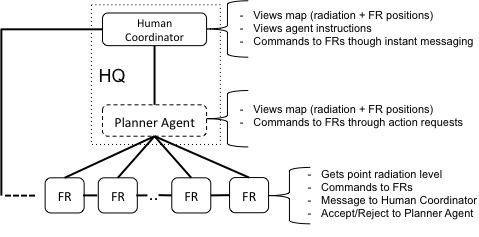
\includegraphics[width=\columnwidth]{scenario.jpg}\vspace{-5mm}
%
%\label{fig:scenario}
%\caption{The interactions between different actors in the disaster scenario. Lines represent communication links. Planner agent and coordinator sit in the headquarters (HQ). First responders (FRs) can communicate with all actors directly.}\end{figure}
\subsection{Human-Agent Collaboration}
\noindent In line with practice in many countries, we assume that the first responders are coordinated from a headquarters (HQ) headed by a human coordinator $H$. In our case, $H$ may be assisted by an autonomous task planning agent $PA$ (more details in Section \ref{sec:algo}), that can receive input from, and direct, the first responders.   Both  $H$ and $PA$  can communicate their  instructions (task plans to pick up targets) directly to the responders using an instant messaging system (or walkie talkie).  While these instructions may be in natural language for $H$, $PA$ instructs them with simple requests such as ``Pick up target X at position Y with team-mates Z'' messages. In turn, the responders may not want to do some tasks (for reasons outlined above) and may therefore simply accept or reject the received instruction from $PA$ or $H$.\footnote{While some agencies may be trained to obey orders (e.g., military or fire-fighting), others (e.g., transport providers or medics) may not be trained to do so.} However, $H$ can query the responders' decisions and request  more information about their status (e.g., fatigue or health) and goals (e.g., meeting with team-mate at position X or going for task Y). Instead, if a task is rejected by the responders, $PA$ records this as a constraint on its task allocation procedure (see details in Section \ref{sec:adaptive}) and returns a new plan. Thus on the one hand, richer interactions are possible between $H$ and the first responders than between them and $PA$. On the other hand, $PA$ runs an sophisticated task allocation algorithm that can compute an efficient allocation, possibly better than the one computable by $H$ (particularly when many responders need to be managed). 

It is important to note that our model captures different types of flexible control: (i) agent-based: when $PA$ directly instructs the responders  and they can use multiple iterations of accept/reject to collaboratively converge to a definite  plan (ii) human-based: when $H$ communicates goals to the responders in open-ended interactions that may permit $H$ to gain a better understanding of the context than $PA$ and therefore formulate corrective measures faster. Moreover, in contrast to previous work that suggested \emph{transfer-of-control} regimes \cite{scerri:etal:2005}, our approach does not constrain transfers of control to target specific decision points in the operation of the system. Rather, our interaction mechanisms are designed (see Section \ref{sec:atomicorchid}) to allow human control at any point (and our results  in Section \ref{sec:evaluation} validate this approach). 

\subsection{The Optimisation Problem}
\label{sec:model}
\noindent Previous agent-based models for team coordination in disaster response typically assume deterministic task executions and environments \cite{ramchurn:etal:2010,Scerri2005}. However, in order to evaluate agent-guided coordination in a real-world environment, it is important to consider uncertainties due to player behaviours and the environment (as discussed in the previous section). Given this, we propose a new representation for the task allocation problem in disaster response that does take into account such uncertainties. More specifically, we represent this problem using an MMDP that captures the uncertainties of the radioactive cloud and the responders' behaviours. We model the spreading of the radioactive cloud as a random process over the disaster space and allow the actions requested from the responders to  fail (because they decline to go to a  task) or incur delays (because they are too slow) during the rescue process. Thus in the MMDP model, we represent  task executions as stochastic processes of state transitions, while the uncertainties of the radioactive cloud and the responders' behaviours can be easily captured with transition probabilities.  More formally, the MMDP is
represented by tuple $\mathcal{M} = \langle I, S, \{A_i\}, P, R
\rangle$, where $I$ is the set of actors as defined in the previous
section,  $S$ is the state space, $A_i$ is a set of responder
$p_i$'s actions, $P$ is the transition function, and $R$ is the
reward function. We elaborate on each of these below.

In more detail, $S= S^G_r \times S_{p_1} \times \cdots \times
S_{p_n} \times S_{t_1} \times \cdots \times S_{t_m}$ where $S^G_r =
\{l_{(x,y)}| (x, y) \in G\}$ is the state variable of the
radioactive cloud that specifies the radioactive level
$l_{(x,y)}\in[0, 100]$ at every point $(x, y)\in G$. $S_{p_i} =
\langle h_i, (x_i, y_i), t_j \rangle$ is the state variable for
each responder $p_i$ that specifies her health level
$h_i\in[0, 100]$, her present position $(x_i, y_i)$, and the task
$t_j$ she is carrying out. $S_{t_j} = \langle {\tt st_j}, (x_j, y_j)
\rangle$ is then the state variable for task $t_j$ to specify its
status ${\tt st_j}$ (i.e., the target is picked up, dropped off, or idle) and position $(x_j, y_j)$. 

The three types of actions  (in set $A_i$) a responder can take
are: (i) {\em stay} in the current location $(x_i, y_i)$, (ii) {\em
move} to the 8 neighbouring locations, or (iii) {\em complete} a
task located at $(x_i, y_i)$. A joint action $\vec{a}=\langle a_1,
\cdots, a_n \rangle$ is a set of actions where $a_i\in A_i$, one
for each responder (a responder may just \emph{stay} at its current
position if it has no targets to rescue). The transition function
$P$ is defined in more detail as: $P= P_r \times P_{p_1} \times
\cdots \times P_{p_n} \times P_{t_1} \times \cdots \times P_{t_m}$
where:
\begin{itemize}
    \itemsep=-2pt
    \item $P_r(s'_r|s_r)$ is the probability the radioactive
        cloud spreads from state $s_r\in S^G_r$ to $s'_r\in
        S^G_r$. It captures the uncertainty of the  radiation
        levels in the environment due to  noisy sensor readings
        and the variations in wind speed and direction.
    \item $P_{p_i}(s'_{p_i}|s, a_i)$ is the probability
        responder $p_i$ transitions to a new state $s'_{p_i}\in
        S_{p_i}$ when executing action $a_i$. For example, when
        a responder is asked to go to a new location,  she
        may not end up there because  she is tired,
        gets injured, or receives radiation doses that are life
        threatening.
    \item $P_{t_j}(s'_{t_j}|s, \vec{a})$ is the probability
        of task $t_j$ being completed. A task $t_j$ can only be completed by a
        team of responders with the required types ($\Theta_{t_j}$) located at the
        same position as $t_j$.
\end{itemize}

Now,  if  $t_j$ is completed (i.e., in ${\tt st_j}\in S_{t_j}$, the
status ${\tt st_j}$ is marked as ``dropped off'' and its position $(x_j,
y_j)$ is within a safe zone), the team will be rewarded using
function $R$. The team is penalised if a responder $p_i$ gets
injured or receives a high dose of radiation (i.e., in $s_{p_i}$,
the health level $h_i$ is 0). Moreover, we attribute a cost to each
of the responders' actions since  each  action requires them to
exert some effort (e.g., running or carrying objects).


Give the above definitions, a policy for the MMDP is a mapping from
states to joint actions, $\pi: S \rightarrow \vec{A}$ so that the
responders know which actions to take given the current state of
the problem. The quality of a policy $\pi$ is  measured by
its expected value $V^\pi$, which can be computed recursively by
the Bellman equation:
\begin{equation}
  V^\pi(s^\tau) = R(s^\tau, \pi(s^\tau)) + \!\!\!\sum_{s^{\tau+1}\in S}\!\!\!
  P(s^{\tau+1}|s^\tau, \pi(s^t)) V^\pi(s^{\tau+1})
\end{equation}
where $\tau$ denotes the current time point and $\pi(s^\tau)$ is a joint action given $s^\tau$. The goal of solving
the MMDP is to find an optimal policy $\pi^*$ that maximises the
expected value with the initial state $s^0$, $\pi^* =
\arg\max_{\pi} V^\pi(s^0)$.

At each decision step, we assume the planning agent can fully
observe the state of the environment $s$ by collecting sensor
readings of the radioactive cloud and GPS locations of the
responders. Given a policy $\pi$ of the MMDP, a joint action
$\vec{a}=\pi(s)$ can be selected and broadcast to the responders
(as mentioned earlier).


%\section{Team Coordination Algorithm}\label{sec:algo}
\noindent Unfortunately, our  MMDP model results in a very large search space,
even for small-sized problems. For example, with 8 responders and
17 tasks in a 50$\times$55 grid, the number of possible states is
more than $2\times 10^{400}$. Therefore, it is practically
impossible to compute the optimal solution. In such cases, we need
to consider approximate solutions that result in high quality
allocations.  To this end, we develop an
approximate solution using  the observation that responders first need to {\em cooperatively}  form teams (i.e., agree on who will do what),
and  that they can then {\em independently} compute the best path to the task.
In our planning algorithm, we use this observation to decompose the
decision-making process into a hierarchical structure with two
levels: at the top level, a task planning algorithm is run for the
whole team to assign the best task to each responder given the
current state of the world; at the lower level, given a task, a
path planning algorithm is run by each responder to find the best
path to the task from her current location.

Furthermore, not all states of MMDPs are relevant to the problem
(e.g., if a responder gets injured, she is incapable of doing any
task in the future and therefore her state is irrelevant
to other responders) and we only need to consider the reachable
states given the current global state $S$ of the problem. Hence,
given the current state, we compute the policy online only for
reachable states. This saves a considerable amount of computation
because the size of the reachable states is usually much smaller
than the overall state space. For example, given the current
location of a responder, the one-step reachable locations are the 8
neighbouring locations plus the current locations, which are 9
locations out of the 50$\times$55 grid. Jointly, the reduction is
huge, from $(50\times 55)^8$ to $9^8$ for 8 responders. Another
advantage of online planning is that it allows us to refine the
model as more information is obtained or unexpected events happen.
For example, given that the wind speed or  direction 
 may change, the uncertainty about the radioactive cloud may increase.
If a responder becomes tired, the outcome of  her actions may
be liable to greater uncertainty.

The main process of our online hierarchical planning algorithm is
outlined in Algorithm~\ref{alg:coordination}. The following
sections describe the procedures of each level in more detail.

\begin{algorithm}[t]
  \caption{Team Coordination Algorithm}\small
  \label{alg:coordination}
  \Indm
  \KwIn{the MMDP model and the current state $s$.}
  \KwOut{the best joint action $\vec{a}$.}
  \Indp\BlankLine
  \tcp{The task planning}
  $\{ t^i \} \gets$ compute the best task for each responder $p_i\in I$ \;
  \ForEach{$p_i\in I$} {
    \tcp{The path planning}
    $a_i \gets$ compute the best path to task $t^i$ \;
  }
  \Return{$\vec{a}$}\vspace{-1mm}
\end{algorithm}


\subsection{Task Planning}
\label{sec:taskplanning}
\noindent As described in Section \ref{sec:model}, each responder
$p_i$ is of a specific type $\theta_i \in \Theta$ that determines which task
she can perform and  a task $t$ can only be completed by a team of
responders with the required types $\Theta_t$. If, at some point in
the execution of a plan, a responder $p_i$ is incapable of
performing a task (e.g., because she is tired or suffered a high
radiation dose), she will be removed from the set of responders
under consideration (that is $I \to I \setminus p_i$). This
information can be obtained from the state $s \in S$. When a task
is completed by a chosen team, the task is simply removed from the
set (that is $T \to T\setminus t_k$ if $t_k$ has been completed).

Now, to capture the efficiency of groupings of responders at
performing tasks, we define the value
of a team $v(C_{jk})$ that reflects the level of performance of
team $C_k$ in performing task $t_j$. This is computed from the estimated rewards the team obtains for performing $t_j$ (as we show below).  Then, the goal of the task
planning algorithm is to assign a task to each team that maximises
the overall team performance given the current state $s$, i.e.,
$\sum_{j=1}^m v(C_{j})$ where $C_j$ is a team for task $t_j$ and $\{
C_1, \cdots, C_m \}$ is a {\em partition} of $I$ ($\forall j\neq
j', C_j \bigcap C_{j'} = \emptyset$ and $\bigcup_{j=1}^m C_j=I$).
In what follows, we first detail the procedure to compute the value
of all teams that are valid in a given state and then proceed to
detail the main algorithm to allocate tasks. Note that these
algorithms take into account the uncertainties captured by the
transition function of the MMDP.


\subsubsection{Team Value Calculation}
\noindent The computation of  $v(C_{jk})$ for each team
$C_{jk}$ is challenging because not all tasks can be completed by
one allocation (there are usually more targets than responders). Moreover, the policy after completing task $t_j$ must also be computed by the agent, which is time-consuming given the number of states and joint
actions. Given this, we propose to estimate $v(C_{jk})$ through
several simulations. This is much cheaper computationally as it avoids computing the complete policy to come up
with a good estimate of the team value, though we may not be able to
evaluate all possible future outcomes. According to the central
limit theorem, if the number of simulations is sufficiently
large, the estimated value will converge to the true $v(C_{jk})$.
This process is outlined in Algorithm~\ref{alg:taskplanning}.
\begin{algorithm}[htbp]\small
  \caption{Team Value Calculation}
  \label{alg:taskplanning}
  \Indm
  \KwIn{the current state $s$,
  a set of unfinished tasks $T$,
  and a set of free responders $I$.}
  \KwOut{a task assignment for all responders.}
  \Indp\BlankLine
  $\{ C_{jk} \} \gets$ compute all possible teams of $I$ for
  $T$ \;
  \ForEach{$C_{jk} \in \{C_{jk}\}$}{
    \tcp{The $N$ trial simulations}
    \For{$i=1$ \KwTo $N$}{
        $(r, s') \gets$ simulate the process with the starting state $s$
        until task $k$ is completed by the responders in $C_{jk}$ \;
        \If{$s'$ is a terminal state} {
            $v_i(C_{jk}) \gets r$ \;
        } \Else {
            $V(s') \gets$ estimate the value of $s'$ with MCTS \;
            $v_i(C_{jk}) \gets r + \gamma V(s')$ \;
        }
    }
    $v(C_{jk}) \gets \frac{1}{N} \sum_{i=1}^{N} v_i(C_{jk})$ \;
  }
  \Return the task assignment computed by Equation~\ref{eq:cf}
\end{algorithm}

In each simulation of Algorithm~\ref{alg:taskplanning}, we first
assign the responders in $C_{jk}$ to task $t_j$ and run the
simulator starting from the current state $s$ (Line 4). After task
$t_j$ is completed, the simulator returns the sum of the rewards
$r$ and the new state $s'$ (Line 4). If all the responders in
$C_{jk}$ are incapable of doing other tasks (e.g., suffered
radiation burns), the simulation is terminated (Line
5). Otherwise, we estimate the expected value of $s'$ using
Monte-Carlo Tree Search (MCTS)~\cite{kocsis2006bandit} (Line 8),
which provides a good trade-off between exploitation and exploration
of the policy space and has been shown to be efficient for large
MDPs.\footnote{Other methods such as sequential greedy assignment
or swap-based hill climbing~\cite{proper2009solving} may also be useful. However, they do not explore the policy space as well as MCTS.} After $N$ simulations, the average value is returned as an approximation of
the team value (Line 10).

The basic idea of MCTS is to maintain a search tree where each node
is associated with a state $s$ and each branch is a task assignment
for all responders. To implement MCTS, the main step is to compute
an assignment for the free responders (a responder is free when she
is capable of doing tasks but not assigned to any) at each
node of the search tree. This can be computed by
Equation~\ref{eq:cf} using the team values estimated by the UCB1
heuristic~\cite{auer2002finite} to balance exploitation and
exploration:
\begin{equation}\small
  v(C_{jk}) = \overline{v(C_{jk})} + c\sqrt{\frac{2N(s)}{N(s, C_{jk})}}
\end{equation}
where $\overline{v(C_{jk})}$ is the averaged value of team $C_{jk}$
at state $s$ so far, $c$ is a trade-off constant, $N(s)$ is the
visiting frequency of state $s$, and $N(s, C_{jk})$ is the
frequency that team $C_{jk}$ has been selected at state $s$.
Intuitively, if a team $C_{jk}$ has  a higher average value in the
trials so far or is rarely selected in the previous visits, it has
higher chance of being selected in the next visit of the tree node.

As we assume that the type of a responder and the role requirements
of each task are static, we can compute all possible team values
offline. Therefore, in the online phase, we only need to filter out
the teams for completed tasks and those containing
incapacitated responders to compute the team set $\{ C_{jk} \}$.

\subsubsection{Coordinated Task Allocation}
\noindent Given the team values computed above, we then solve the
following optimisation problem to find the best solution:
\begin{equation}
  \begin{array}{lll}
    \max\limits_{x_{jk}} & \sum_{j, k} x_{jk} \cdot v(C_{jk}) & \\[2pt]
    \mbox{s.t.} & x_{jk} \in \{0, 1\} & \\[2pt]
    & \forall j, \sum_{k} x_{jk} \leq 1 & \mbox{(i)} \\[2pt]
    & \forall i, \sum_{j, k} \delta_i(C_{jk}) \leq 1 & \mbox{(ii)}
  \end{array}
  \label{eq:cf}
\end{equation}
where $x_{jk}$ is the boolean variable to indicate whether team
$C_{jk}$ is selected for task $t_j$ or not, $v(C_{jk})$ is the value of team $C_{jk}$, and $\delta_i(C_{jk}) =
1$ if responder $p_i\in C_{jk}$ and 0 otherwise. In the
optimisation, constraint (i) ensures that a task $t_j$ is allocated
to at most one team (a task does not need more than one group of
responders) and constraint (ii) ensures that a responder $p_i$ is
assigned to only one task (a responder cannot do more than one task
at the same time). This is a standard Mixed Integer Linear Program
(MILP) that can be efficiently solved  using solvers (e.g., IBM CPLEX or lp\_solve).

\subsubsection{Adapting to Responder Requests}\label{sec:adaptive}
\noindent An important characteristic of our approach is that it can easily
incorporate the preferences of the responders. For example, if a
responder declines a task allocated to it by the planning agent, we
simply filter out the teams for the task that contain this
responder. By so doing, the responder will not be assigned to the
task. Moreover, if a responder prefers to do the tasks with another
responder, we can increase the weights of the teams that
contain them in Equation~\ref{eq:cf} (by default, all teams
have identical weights of 1.0). Thus, our approach is adaptive to the
 preferences of human responders.

\subsection{Path Planning}
\label{sec:pathplanning}

\noindent In the path planning phase, we compute the best path for
a responder to her assigned task. This phase is stochastic as there
are uncertainties in the radioactive cloud and the responders'
actions. We model this problem as a single-agent MDP that can be
defined as a tuple, $\mathcal{M}_i = \langle S_i, A_i, P_i, R_i
\rangle$, where: (1) $S_i = S^G_r \times S_{p_i}$ is the state
space, (2) $A_i$ is the set of $p_i$'s actions, (3) $P_i = P_r
\times P_{p_i}$ is the transition function, and (4) $R_i$ is the
reward function. In this level, responder $p_i$ only needs to
consider the states of the radioactive cloud $S^G_r$ and her own
states $S_{p_i}$ and her moving actions. Similarly, the transition
function only needs to consider the spreading of the radioactive
cloud $P_r$ and the changes of her locations and health levels when
moving in the field $P_{p_i}$, and the reward function only needs
to consider the cost of moving to a task and the penalty of
receiving high radiation doses. This is a typical MDP that can be
solved by many existing solvers (see the most recent
survey~\cite{kolobov2012planning}). We choose Real-Time Dynamic
Programming (RTDP)~\cite{barto1995learning} because it is simple
and particularly fits our problem, that is, a goal-directed MDP
with large number of states. However, other approaches for solving
large MDPs  could equally be used here.

There are several techniques we use to speed up the convergence of
RTDP. In our problem, the map is static. Thus, we can initialize
the value function $V(s)$ using the cost of the shortest path
between the current location and the task location on the map, which
can be computed offline without considering the radioactive cloud.
This helps RTDP quickly navigate among the obstacles (e.g.,
buildings, water pools, blocked roads) without getting trapped in
dead-ends during the search. Another speed up is also possible if,
when traversing the possible states, we only consider the
responder's current location and the neighbouring points. This will
further speed up the algorithm where the main bottleneck is the
huge state space.

\subsection{Simulation Results}

%\begin{figure}[htbp]
%  \centering
%  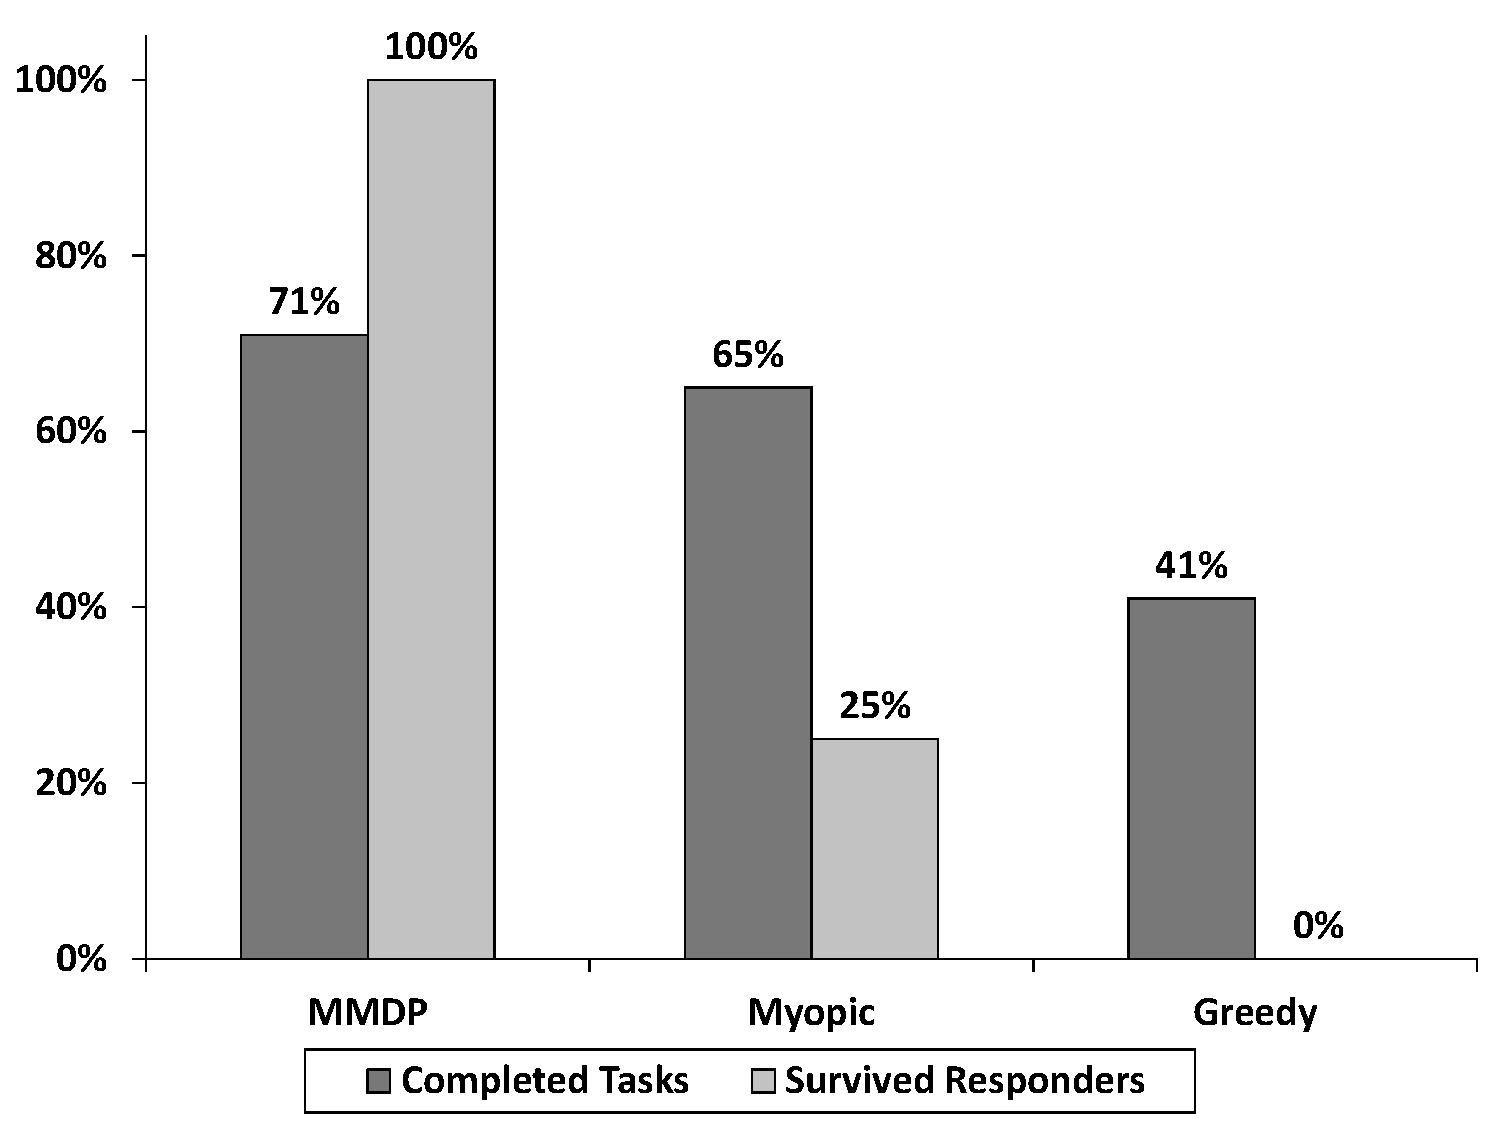
\includegraphics[width=0.8\linewidth]{simulation}
%  \caption{Experimental results for the MMDP, myopic, greedy
%  algorithms in simulation.}
%  \label{fig:simulation}
%\end{figure}


\noindent Before deploying our solution (as part of $PA$) to advise
human responders, it is important  to test its performance to
ensure it can return efficient solutions on simulations of the
real-world problem. Given there is no extant solution that
takes into account uncertainty in team coordination for emergency
response, we compare our algorithm with a greedy and a
myopic method to evaluate the benefits of coordination and
lookahead. For each method, we use our path planning algorithm to
compute the path for each responder. In the greedy method, the responders
are uncoordinated and select the closest tasks they can do. In
the myopic method, the responders are coordinated to select the
tasks but have no lookahead for the future tasks (Line 8 in
Algorithm~\ref{alg:taskplanning}). Table~\ref{tab:simulation} shows
the results for a problem with 17 tasks and 8 responders on a
50$\times$55 grid. As can be seen, our MMDP algorithm 
completes more tasks than the myopic and greedy methods (see Table
\ref{tab:simulation}). More importantly, our algorithm guarantees
the safety of the responders, while in the myopic method  only 25\%
of the responders survive and in the greedy method all responders
are killed by the radioactive cloud. More extensive evaluations are
beyond the scope of this paper as our focus here is on the use of
the algorithm in a field deployment to test how humans take up
advice computed by the planning agent $PA$.
\begin{table}[htbp]
  \centering
  \caption{Experimental results for the MMDP, myopic, greedy
  algorithms in simulation.}
  \begin{tabular}{l|c|c|c}
   & MMDP & myopic & greedy \\
  \hline
  No. of completed tasks & 71\% & 65\% & 41\% \\
  \hline
  No. responders alive at the end & 100\% & 25\% & 0\% \\
  \end{tabular}
  \label{tab:simulation}\vspace{-3mm}
\end{table}

\section{The A\lowercase{tomic}O\lowercase{rchid} Game}\label{sec:atomicorchid}
\noindent The AtomicOrchid game was used to embed the planning agent in order to trial mixed-initiative coordination.
We adopt a serious mixed-reality games approach to counteract the limitations of computational simulations \cite{Fischer:etal:2012}. The impact of emotional and physical responses, such as stress, fear, exertion or panic remains understudied in approaches that rely purely on computational simulation \cite{drury:etal:2009}. For example, \citeauthor{simonovic:2009} (\citeyear{simonovic:2009}) highlights that simulations may not account for ``human psychosocial characteristics and individual movement, and (...) learning ability''. In contrast, our approach creates a realistic setting in that participants experience physical exertion and stress through bodily activity and time pressure, mirroring aspects of a real disaster setting \cite{paho:2001}. This, in turn, provides greater confidence in the efficacy of behavioural observations of team coordination.

In more detail, AtomicOrchid is a location-based mobile game based on the fictitious scenario described earlier. First responders are assigned a specific type: medic, fire-fighter, soldier, or transporter. Their mission is to evacuate all four types of targets: victim (requires medic and fire-fighter), animal (requires medic and transporter), fuel (requires soldier and fire-fighter), or other resource (requires soldier and transporter) before they are engulfed by the radio-active cloud.\footnote{The radiation cloud diffusion process is modelled using the Smoluchowski drift-diffusion equation. Details are given in the supplemental material.}  The first responders are supported by (at least) one person $H$ in a centrally located HQ room, and the planning agent $PA$ that sends the next task (as described in the previous section) to the team of first responders. A video of AtomicOrchid can be viewed at: {\small \url{http://bit.ly/1ebNYty}}.

\subsubsection{Player Interfaces.}
\noindent First responders are equipped with a `mobile responder tool' providing sensing and awareness capabilities in three tabs (geiger cou\-nter, map, messaging and tasks; see Figure \ref{fig:ui}). The first tab shows a reading of radioactivity, player health level (based on exposure), and a GPS-enabled map to locate fellow responders, the targets to be rescued and the drop off zones for the targets. The second tab provides a broadcast messaging interface to communicate with fellow first responders and the HQ. The third tab shows the team and task allocation dynamically provided by the agent $PA$ that can be accepted or rejected. Notifications are used to alert both to new messages and task allocations.

\begin{figure}[htbp]
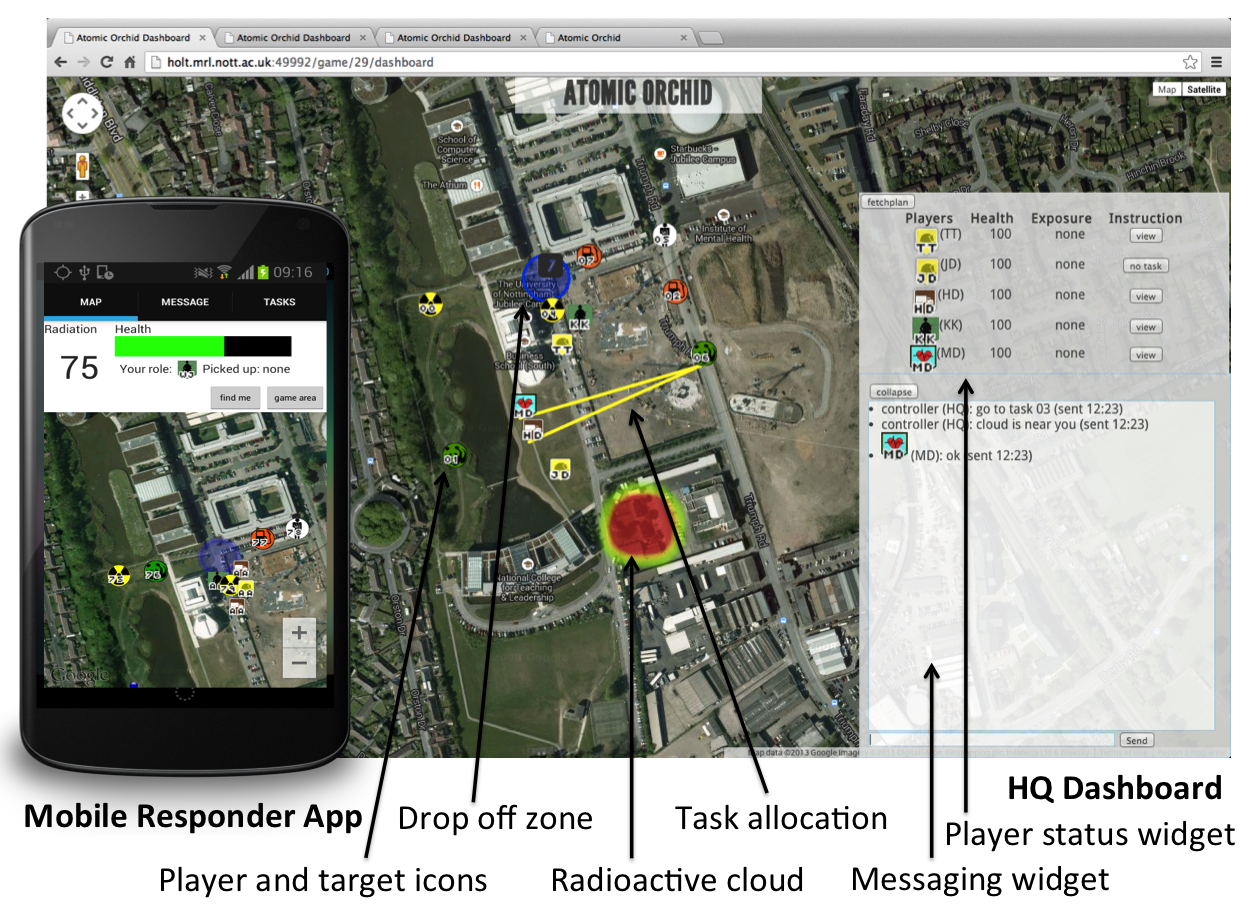
\includegraphics{UI.png}
\caption{Mobile first responder and HQ interfaces.}\label{fig:ui}
\end{figure}

$H$ has at her disposal an `HQ dashboard' that provides an over\-view of the game area, including real-time information of the players' locations (see Figure \ref{fig:ui}). The dashboard provides a broadcast messaging widget, and a player status widget to monitor the responders' exposure and health levels. $H$ can further monitor the current team and task allocations to individual responders by $PA$ (by clicking on a button). Crucially, only $H$ and $PA$ have a view of the radioactive cloud, graphically depicted as a heatmap (`Hotter' (red) zones correspond to higher levels of radiation).

%\subsection{System Architecture}
 AtomicOrchid is based on the geo-fencing game MapAttack. The location-based game is underpinned by a client-server architecture that relies on real-time data streaming between client and server for frequent events (e.g., location updates and radiation exposure). In this way, first responders are kept informed in near real-time. Finally,  to build the mobile app, we adapted the existing MapAttack Android app.

%The platform is built using the geoloqi platform, Sinatra for Ruby, and state-of-the-art web technologies such as socket.io, node.js and the Google Maps API. 

\subsubsection{Integrating the Planning Agent.}
\noindent The planning agent $PA$ takes the game status (i.e., positions of players, known status of the cloud, and messages received from players) as input and produces a plan for each responder  for the current state.  The AtomicOrchid server requests a plan from the agent by transmitting the game status. Polling (and thus re-planning) is triggered by two types of game events:
\begin{itemize}
\item \textit{Completion of task}. On successful rescue of a target, a new plan (i.e., allocation of tasks to each responder) is requested from the agent.
\item \textit{Explicit reject}. On rejection a task by any of the first responders, a new plan is requested. The rejected allocation is used to constrain the set of solutions returned. For example, if two responders (a medic and a soldier) were allocated a task and the medic rejected it, $PA$ would search for an  allocation with the constraint that this medic should not be allocated this task.
\end{itemize} 

%\subsection{Interacting with planning agent}
%There can interact directly with field players through a task tab (Figure xx) and agent plans are also visible to HQ's dashboard interface.
Once a plan is received from $PA$, the AtomicOrchid game engine splits the plan  for a given team (i.e., $C_{jk}$ for task $t_j$ and team $C_k$) into individual task allocations for each player (e.g., $i_1$ and $i_2$ to $t_j$ where $C_k = \{i_1,i_2\}$)  and sends them to their mobile responder app. The app presents the task allocation in the task tab, detailing: i) the responder to team up with, ii) the allocated target (using target id), and iii) approximate direction of the target (e.g., north, east).  %Once a player accepts a task, an acknowledgement is sent to their teammate, while rejecting a task triggers a new assignment from $PA$. 

%Furthermore, $H$ is provided with a visualisation of task allocations for each player on demand (by button press), to help monitor the task allocation computed by the agent.


%\subsection{Radiation Cloud Modelling}\label{sec:radiation}
\noindent The radiation cloud is assumed to be monitored using a number of sensors on the ground (within the disaster space) that collect readings of the radiation cloud intensity and wind velocity every minute of the game. These sensors can be at fixed locations or held by mobile agents.  The radiation cloud diffusion process is modelled using the Smoluchowski drift-diffusion equation, 
\begin{eqnarray*}
\frac{D \text{Rad}({\bf z}, \tau)}{D \tau}=\kappa \triangledown^2 \text{Rad}({\bf z},\tau)-\text{Rad}({\bf z},\tau)\triangledown \cdot {\bf w}({\bf z},\tau)+\sigma({\bf z},\tau)
\end{eqnarray*}
where $D$ is the material derivative, $\text{Rad}({\bf z},\tau)$ is the radiation cloud intensity at location ${\bf z}=(x,y)$ at time $\tau$, $\kappa$ is a fixed diffusion coefficient and $\sigma$ is the radiation source(s) emission rate. %The diffusion equation is solved on a regular grid defined across the environment with grid coordinates $G$ (as defined in Section \ref{sec:model}).  Furthermore, the grid is solved at discrete time instances $\tau$.  The cloud is driven by stochastic wind forces which vary both spatially and temporally.  These forces induce anisotropy into the cloud diffusion process  proportional to the local average wind velocity, ${\bf w}({\bf z},\tau)$.  The wind velocity is drawn from two independent Gaussian processes (GP), one GP for each Cartesian coordinate axis, $w_i({\bf z},\tau)$, of ${\bf w}({\bf z},\tau)$.  The GP captures both the spatial distribution of the wind velocity and the dynamic process resulting from shifting wind patterns (e.g., short term gusts and longer term variations). 

% In our simulation, each spatial wind velocity component is modelled by a squared-exponential GP covariance function, $K$, with fixed input and output scales (although any covariance function can be substituted). Furthermore, as wind conditions may change over time we introduce a temporal correlation coefficient, $\rho$, to the covariance function.  Thus, for a single component, $w_i$, of ${\bf w}$, defined over grid $G$ at times $\tau$ and $\tau^\prime$, the wind process covariance function is, $\text{Cov}(w_i(G,\tau),w_i(G,\tau^\prime))=\rho(\tau,\tau^\prime) K(G,G)$.  We note that, when $\rho=1$ the wind velocities are time invariant (although spatially variant).  Values of $\rho<1$ model wind conditions that change over time.

Using this model, we are able to create a moving radiation cloud. This poses a real challenge both for the HQ ($PA$ and $H$) and the responders on the ground, as the predictions they make of where the cloud will move to will be prone to uncertainty both due to the simulated wind speed and direction. 


%(\textbf{Steve: in the platform we take the `real' values from the diffusion process i believe. Does the above capture this? We will say that we will add the features you mention below to a future version of the platform where we aim to do both situational awareness and rescue. Add a sentence above to conclude where we took the values from and the process takes into account the  location of radiation source. Also, your notation clashes with the notations in the scenario and Feng's algorithm - please try to align.}
%The cloud intensity and wind velocity are measured by {\it monitor agents} equipped with geiger-counters and anemometers.  These agents are directed to take measurements with greatest information gain in the radiation cloud intensity.  The measurements are folded into the EKF and this refines estimates of the radiation cloud across the grid.  Figure~\ref{radiation_screen_shots} shows example cloud simulations for slow varying (i.e. $\rho=0.99$) and gusty (i.e. $\rho=0.90$) wind conditions.  Figure~\ref{radiation_screen_shots}(a) shows slow varying wind conditions in which case the radiation cloud can be interpolated accurately using sparse sensor measurements and the LFM model.  Alternatively, during gusty conditions the radiation cloud model is more uncertain far from the locations where recent measurements have been taken, as shown in Figure~\ref{radiation_screen_shots}(b).
%
%\begin{figure}[ht] \begin{center}
%    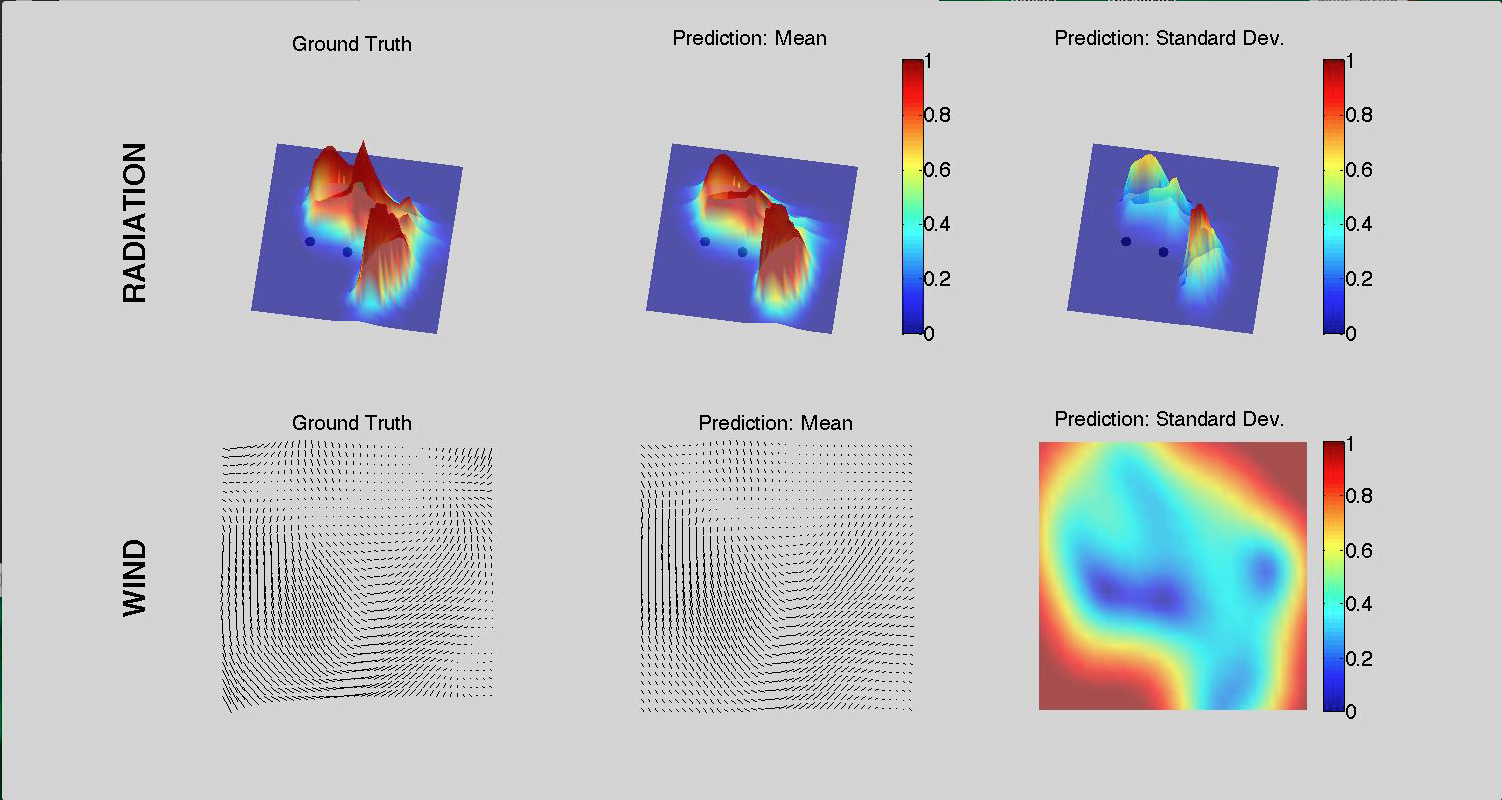
\includegraphics[width=0.45\textwidth]{figures/radiation_ss_calm.png}\\
%    (a) Slowly varying wind conditions\\ \ \\
%    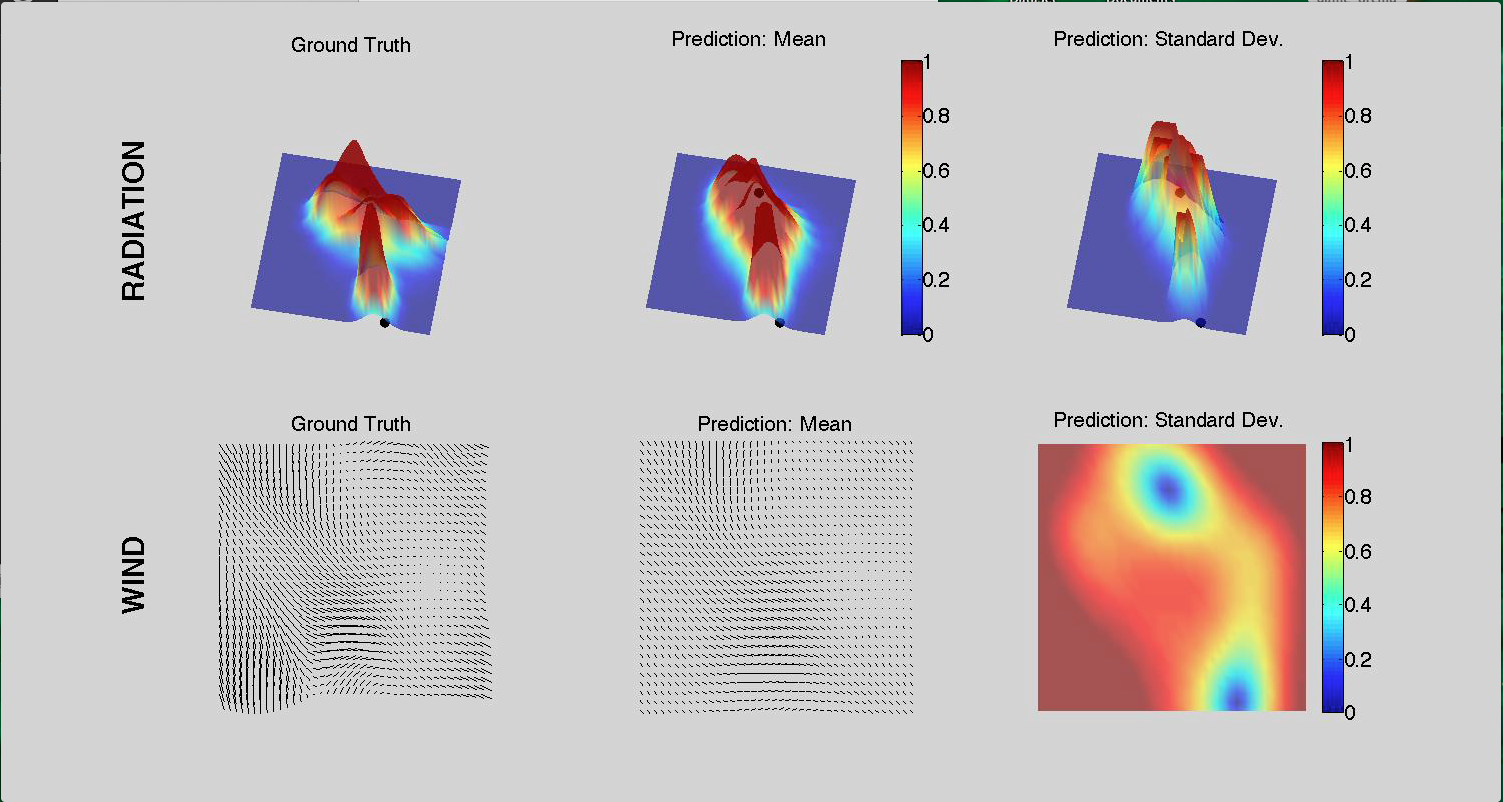
\includegraphics[width=0.45\textwidth]{figures/radiation_ss_gust.png}\\
%    (b) Gusty wind conditions 
%\caption{\label{radiation_screen_shots} Radiation and wind simulation ground truth and EKF estimates obtained using measurements from monitor agents (black dots).  Left most panes are ground truth radiation and wind conditions, the middle panes are corresponding estimates and right most panes are state uncertainties:  (a) Invariant and (b) gusty wind conditions.}
%\end{center}
%\end{figure}

\section{The Field Trials}\label{sec:evaluation}
\noindent We ran three sessions of AtomicOrchid with participants recruited from the local university. We focus on situated reactions to agent instructions to explore how the interaction unfolded. The uncertainties of the field setting and small number of trials prohibit statistical analysis at this stage. Hence, we focus on descriptive results. 

%\subsection{Participants and Procedure}
%\noindent  
A total of 24 participants (13 males and 11 females) were recruited through posters and emails, and reimbursed with \pounds 15  for 1.5-2 hours of study. The majority were students. The procedure consisted of 30 minutes of game play, and about 1 hour in total of pre-game briefing, consent forms,  a short training session, and a post-game group discussion. 

%Upon arrival in the HQ (set up in a meeting room at the local university), participants were briefed and asked to consent to participate. They were presented with a demographic questionnaire to record gender, occupation, experience of using smartphones and level of map navigation skills.

At the end of the briefing, in which mission objectives and rules were outlined, responder types were randomly assigned to all participants (fire-fighter, medic, transporter, soldier). The HQ was staffed by a different member of the research team in each session in order to mimic an experienced $H$, while avoiding the same person running the HQ every time.  Moreover, responders were provided with a smartphone and $H$ with a laptop. The team was given 5 minutes to discuss a common game strategy.  First responders were then accompanied to the starting point within the designated game area, about 1 minute walk from $H$. After 30 minutes of game play the first responders returned to the HQ where the post-game group interview was conducted.

%(\textbf{Joel: where did the agent run ? --> Gopal, this should be covered in the previous section I think?})
%\subsection{Game Sessions}
%\noindent 
We ran one session without $PA$, and two sessions with $PA$  to compare team performance in the two versions. Each session involved \emph{different} sets of players (8 each). Thus,  players were unique to a session to avoid learning effects between sessions. We also ran a pilot study for each condition to fine tune game configuration. The whole team was formed such that there were two of each of the four types of responders. The terrain of the 400$\times$400 metres  game area includes grassland, a lake, buildings, roads,  footpaths and lawns. There were two  drop-off zones and 16 targets in each session. There were four targets for each of the four target types. The target locations, pattern of cloud movement and expansion were kept constant for all game sessions. The pilot study showed that this was a challenging, yet not too overwhelming configuration of game area size, and number of targets to collect in a 30 min game session. 

\subsubsection{Data Collection and Analysis.}
\noindent 
We collected more than 4 hours of video and 10 pages of transcribed audio (from game action and at HQ). We then developed a log file replay tool to triangulate video recordings of game action with the timestamped system logs that contain a complete record of the game play, including responders' GPS location, their health status and radioactive exposure, messages, cloud location, locations of target objects and task status.

%Video recordings of field action were catalogued to identify sequences (episodes) of interest (cf. Heath et al., 2010). Key decision points in teaming and task allocation served to index the episodes. Interesting distinct units of interaction were transcribed and triangulated with log files of relevant game activity for deeper analysis. Due to space constraints we can only  present one fragment in this paper to illustrate how human-agent collaboration typically unfolded (TODO).
To assess how humans interact with each other and with $PA$, we focused on collecting data relevant to $PA$'s task allocations and remote messages  that are used to support coordination. In particular, we use speech-act theory \cite{searle:1975} to classify messages sent between and among responders and $H$. We focus on the most relevant types of acts in this paper (which are also the most frequently used):
\begin{itemize}
\item Assertives: \textit{speech acts that commit a speaker to the truth of the expressed proposition}; these were a common category as they include messages that contain situational information.
\item Directives: \textit{speech acts that are meant to cause the hearer to take a particular action}, e.g. requests, commands and advice, including task and team allocation messages. 
\end{itemize}

\subsubsection{Results.}
\noindent Overall, 8 targets were rescued in the non-agent condition (Session A), and respectively 12 targets (Session B) and 11 targets (Session C) were rescued in the agent condition. Teams (re-)formed six times in session A, four times in session B and nine times  in session C. Average player health after the game was much higher (more than double) for the agent-assisted sessions (80 for Session B and 82 for Session C) compared to the session without agent (40 in Session A). In fact, one responder `died' in Session A.
$PA$ dynamically re-planned 14 times in session B and 18 times in session C. This was mainly triggered by a dropped off (completed) target (24 times), but sometimes this was triggered by a player declining the agent's task allocation (8 times). 

%\vspace{-3mm}

\begin{table}[ht]\small\centering
\begin{tabular}{c | c c | c c c c | c}
 & \multicolumn{2}{c|}{no agent} &  \multicolumn{4}{c|}{agent} & Total \\
 \hline
 Speech acts & \multicolumn{2}{c|}{Session A} & \multicolumn{2}{c}{Session B} & \multicolumn{2}{c|}{Session C} & \\
  & HQ & FR & HQ & FR & HQ & FR & \\
  \hline
  Directives & 89 & 0 & 34 & 2 & 34 & 0 & 159 \\
  Assertives & 33 & 6 & 26 & 16 & 24 & 16 & 121 \\
  \hline
  Total & 122 & 6 & 60 & 18 & 58 & 16 & 280 \\
\end{tabular}
%\vspace{-2mm}
 \caption{Message classification. FR: First Responder.} \label{tab:msgs}
\end{table}

%Table \ref{tab:msgs} shows the remote message directives (mainly related to task allocation and execution) and assertives (mainly related to situational awareness) sent in the sessions. 
In what follows, we explicate how the different types of messages (Table \ref{tab:msgs}) were handled to give a sense of mixed-initiative coordination in the sessions.


%\subsubsection{Handling Task Allocations}
In the non-agent condition, $H$ sent 43 task allocation directives (see Figure \ref{fig:msgs}). The field responders brought up only 15 out of these messages in conversation. Out of these 15, responders chose to ignore the instructions only once because they were engaged in another task that they did not want to abandon. A further 4 $H$ instructions were consistent with a decision to rescue a certain target that had already been agreed locally by the responders. In the remaining 10 cases, first responders chose to follow the instructions. Although players were willing to follow $H$'s instructions, they failed to correctly follow the instructions due to confusion and misunderstanding in the communication. In fact, only 2 instances of directives from $H$ led to task completion. The first responders performed 6 rescue operations (tasks) without being instructed by $H$.

\begin{figure}[t]
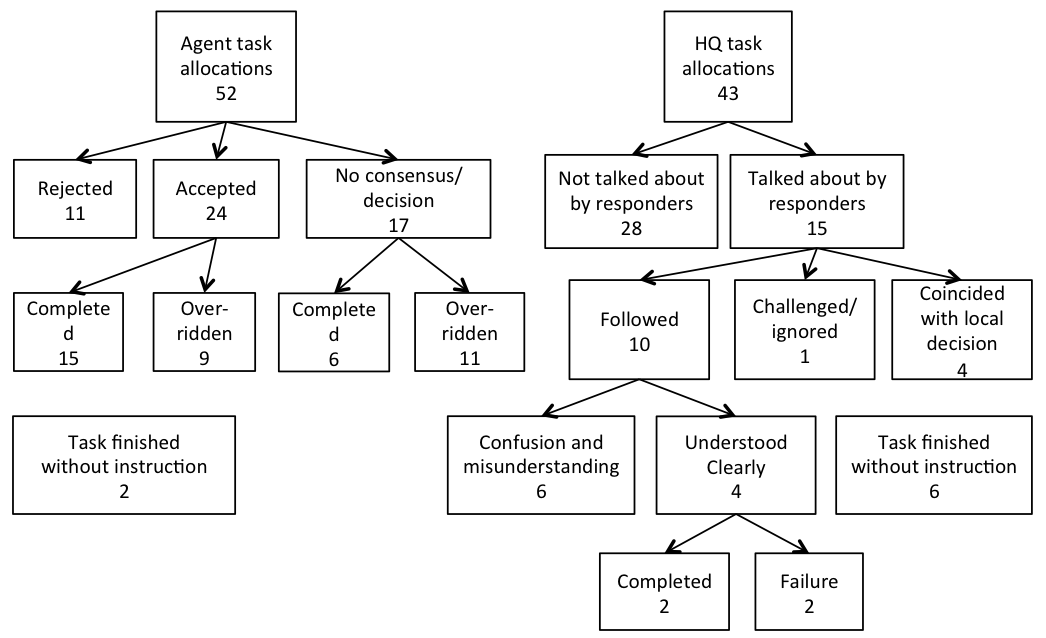
\includegraphics{message_handling.png}
\caption{Message handling by first responders in  agent (left), and non-agent (right) versions.}\label{fig:msgs}
\end{figure}

In contrast, when task allocation was handled by the agent (52 tasks allocated in session B and C), responders explicitly accepted 24 tasks,  of which they completed 15  successfully. Although there was either no response or no consensus between the responders (in 17 tasks allocated), they still completed 6 of these tasks successfully. In total, 20 task allocations were withdrawn by the agent as a result of re-planning. 

%\paragraph{Rejecting task allocations}
In terms of task rejections, first responders rejected $PA$'s task allocation 11 times in the agent version. All of the rejections happened when following the allocation would have \emph{split existing teams}, or instructed responders to team up with \emph{physically more distant responders}. In most cases (9 out of 11), the rejection \emph{adjusted the agent's task allocation} to become consistent with the responder's current team. In the other two cases, the responders rejected the task allocation one more time before receiving the desired task allocation. Notably, for accepted instructions the average distance between suggested teammates was 12 metres. For rejected instructions the average was 86 metres.

The results above show that  the simple mechanism to get $PA$ to re-plan (i.e., reject/accept) was more successful (more tasks completed and less confusion) than the open-ended interactions between $H$ and the responders.  Moreover, the fact that many of the rejections coincided with larger distances to suggested teammates implies that players chose to do the tasks they \emph{preferred} rather than those deemed optimal by the agent. This indicates there may be an issue of trust in the agent, but also that it may be easier for a responder to impose such preferences on an agent (and indirectly to other team members) rather than expressing this to $H$ or directly to teammates. 

% Role of HQ commander
Furthermore, in the agent-assisted setting, $H$ frequently \emph{monitored} the allocation of tasks  returned by the agent (57 clicks on `show task' in UI responder status widget). Whereas 43 directives (out of 89) in the non-agent session were task allocations, in the agent version only 16 out of 68 were directly related to task allocations. Out of these, $H$ directly reinforced the agent's instruction 6 times (e.g., ``SS and LT retrieve 09''), and complemented (i.e., added to or elaborated) $PA$'s task allocation 5 times (e.g., ``DP and SS, as soon as you can head to 20 before the radiation cloud gets there first''). $H$  did `override' $PA$'s instruction in 5 cases.  

In the agent version, most of $H$'s directives (52 out of 68) and assertives (49 out of 50) focussed on \textit{providing situational awareness and routing} the responders to avoid exposing them to radiation. For example, ``NK and JL approach drop off 6 by navigating via 10 and 09.'', or ``Radiation cloud is at the east of the National College''. 

\subsection{Discussion and Conclusions}
\label{sec:discussion}
In summary, the results from our field trials suggest three key observations with regard to  human-agent coordination: 
\begin{enumerate}
\item First responders performed better (rescued more targets)  and maintained higher health levels when supported by the agent.  These results echo those obtained under simulation (shown earlier) and  may reflect the better forward-planning capability of the planning agent compared to human responders and HQ. 
 
\item Rejecting tasks was relatively frequently employed to trigger re-planning to obtain new task allocations aligned with responder preferences.  In each case, the planning agent was able to adapt to provide an alternative  that was acceptable to the responders. Without this facility we believe the responders would have chosen to ignore the plan. Task rejection seemed to be linked to changes to established teams, especially when members were relatively distant. Consequently, these kinds of allocations may need particular support (e.g., explanation) or might be less preferentially selected by $PA$.

\item When task allocation was handled by $PA$, $H$ could focus on providing vital situational awareness to safely route first responders around danger zones: thus demonstrating effective division of labour and complementary collaboration between humans and agents.
\end{enumerate}

Given these observations we argue that a planning agent for team formation should not only model the uncertainty in player behaviours and in the environment, but that interactional challenges also need to be addressed  if such a technology is to be accepted in practice. In particular, if such a system were to be deployed with expert responders, we foresee the need to ensure the agent's recommendations come with proper explanations in order to be trusted and further augment their capability. In particular, we propose the following \textit{design guidelines for human-agent collaboration}:

\noindent \textbf{Adaptivity}:  planning algorithms should be designed to take in human input, and more importantly, be \emph{responsive} to the needs of the users. Players repeatedly requested new tasks and this would not have been possible unless our algorithm  was computationally efficient  and could  assimilate updates, requests, and constraints dynamically. 

\noindent \textbf{Interaction Simplicity}:  agents should be designed with minimal options to simplify the reasoning needed to interact with them, particularly when responders are under pressure to act. $PA$ was designed to issue simple commands (Do X with Y) and respond to simple requests (OK or Reject Task). These were better at guiding players to do the right task than the unstructured human communication (fraught with inconsistencies and inaccuracies) in the non-agent version. 

\noindent \textbf{Flexbile autonomy}: interfaces should be designed to pass control between humans and agents in flexible ways. The HQ dashboard allowed $H$ to \emph{check} and \emph{correct for} the allocations of $PA$, taking into account the real-world constraints that the players on the ground faced. In particular, letting the human oversee the agent (i.e., ``on-the-loop") at times and actively instructing  the players (and bypassing the agent) at other times (i.e., ``in-the-loop") as and when needed, was seen to be particularly effective. In contrast to \cite{scerri:etal:2005} which advocated pre-scripted transfers of control, in our case  control was transferred between $H$ and $PA$ depending on the context and, at times, in unforeseen ways.

To further refine these guidelines, future work will look at running AtomicOrchid with expert responders and explore different interactional arrangements of humans and agents, in particular where control is distributed across the team.\vspace{-1mm}


%\section{Real-world trial}
%We ran three sessions of AtomicOrchid with participants recruited from the local university to trial mixed-initiative coordination in a disaster response scenario. 
%
%\subsection{Participants and procedure}
%A total of 24 participants (7 of them were female) were recruited through posters and emails, and reimbursed with 15 pounds for 1.5-2 hours of study. The majority were students of the local university.
%
%The procedure consisted of 30 minutes of game play, and about 1 hour of pre-game briefing, consent forms and a short training session, and a post-game group discussion. 
%
%%Upon arrival in the HQ (set up in a meeting room at the local university), participants were briefed and asked to consent to participate. They were presented with a demographic questionnaire to record gender, occupation, experience of using smartphones and level of map navigation skills.
%
%At the end of the briefing in which mission objectives and rules were outlined, responder roles were randomly assigned to all participants (fire-fighter, medic, transporter, soldier). HQ was staffed by a different member of the research team in each session in order to mimick an experienced HQ whilst avoiding the same person running HQ every time. 
%
%Field responders were provided with a smartphone; HQ coordinators with a laptop. The team was given 5 minutes to discuss a common game strategy. 
%
%%(\textbf{Joel: where did the agent run ? --> Gopal, this should be covered in the previous section I think?})
%
%Field responders were then accompanied to the starting point within the designated game area, about 1 minute walk from headquarters. Once field responders were ready to start, HQ sent a `game start' message. After 30 minutes of game play the field responders returned to the HQ where a group interview was conducted, before participants were debriefed and dismissed.
%
%\subsection{Game sessions}
%We ran one session without the planner agent, and two sessions with the planner agent to be able to compare team performance in the two versions. We also ran a pilot study for each condition to fine tune game configuration. The 8 field responders in each session were randomly allocated a responder so that the whole team had two of each of the four kinds of responder roles. The terrain of the 400x400metres game area includes grassland, a lake, buildings, roads, and footpaths and lawns. There were two drop off zones and 16 targets in each session. There were four targets for each of the four target types. The target locations, pattern of cloud movement and expansion were kept constant for all game sessions. The pilot study showed that this was a challenging, yet not too overwhelming configuration of game area size, and number of targets to collect in a 30 min game session. 
%
%\subsection{Data collection and analysis}
%We developed a log file replay tool to triangulate video recordings of game action with the time stamped system logs that contain a complete record of the game play, including responders' GPS location, their health status and radioactive exposure, messages, cloud location, locations of target objects and task status.
%
%%Video recordings of field action were catalogued to identify sequences (episodes) of interest (cf. Heath et al., 2010). Key decision points in teaming and task allocation served to index the episodes. Interesting distinct units of interaction were transcribed and triangulated with log files of relevant game activity for deeper analysis. Due to space constraints we can only  present one fragment in this paper to illustrate how human-agent collaboration typically unfolded (TODO).
%
%In this paper we focus on how both agent task allocations and remote messages are used as a coordination resource. We use speech-act theory (Searle, 1975) to classify messages sent between and among responders and HQ. We focus on the most relevant types of acts in this paper (which are also the most frequently used in AtomicOrchid):
%
%\begin{itemize}
%\item Assertives: \textit{speech acts that commit a speaker to the truth of the expressed proposition}; these were a common category as they include messages that contain situational information.
%\item Directives: \textit{speech acts that are meant to cause the hearer to take a particular action}, e.g. requests, commands and advice, including task and team allocation messages. 
%\end{itemize}
%
%\subsection{Results}
%Overall, 8 targets were rescued in the non-agent condition (Session A), and respectively 12 targets (Session B), and 11 targets (Session C) were rescued in the agent condition. Teams (re-)formed six times in session A, four times in session B and nine times  in session C. Average player health after the game was 40/100 in Session B, and 81 for the agent-assisted sessions (B:80, C: 82). One responder `died' in Session A.  
%
%The agent dynamically re-planned 14 times in session B, and 18 times in session C. Most of the times, this was triggered when a target was dropped off in the safe zone (24 times), some times this was triggered by a player rejecting the agent's task allocation (8 times). 
%
%Table \ref{tab:msgs} shows the directives (mainly related to task allocation and execution) and assertives (mainly related to situational awareness) sent in the sessions. The next sections draw on how these messages were handled to give a sense of mixed-initiative coordination in the game sessions.
%
%\begin{table}\footnotesize
%\begin{tabular}{c | c c | c c c c | c}
% & \multicolumn{2}{c|}{no agent} &  \multicolumn{4}{c|}{agent} & Total \\
% \hline
% Speech acts & \multicolumn{2}{c|}{Session A} & \multicolumn{2}{c}{Session B} & \multicolumn{2}{c|}{Session C} & \\
%  & HQ & FR & HQ & FR & HQ & FR & \\
%  \hline
%  Directives & 89 & 0 & 34 & 2 & 34 & 0 & 159 \\
%  Assertives & 33 & 6 & 26 & 16 & 24 & 16 & 121 \\
%  \hline
%  Total & 122 & 6 & 60 & 18 & 58 & 16 & 280 \\
%\end{tabular}
% \label{tab:msgs}
% \caption{Message classification.}
%\end{table}
%
%
%\subsubsection{Handling task allocations}
%Fig. \ref{fig:msgs} shows how field responders handled task allocations in the agent and in the non-agent condition. In the non-agent condition, HQ sent 43 task allocation directives. Out of these, the recipient field responders addressed only 15 messages (bringing them up in conversation). Out of these 15, responders chose to ignore the instructions only once. The responder ignored the instruction because they were engaged in another task and did not want to abandon it. A further 4 HQ instructions were consistent with a decision to rescue a certain target that has already been made locally by the responders. In 10 cases field responders chose to follow the instructions. Although players were willing to follow HQ's instructions, they failed to correctly follow the instructions due to confusion and misunderstanding in the communication. In fact, only 2 instances of directives from the HQ led to task completion.The field responders accomplished task allocation of the other 6 saved targets locally without being instructed by HQ.
%
%On the other hand, when task allocation was handled by the agent, responders accepted 24 tasks, out of which they completed 15 tasks successfully. Even if there was no response or consensus between the responders (in 17 cases), still six out of 17 tasks were completed successfully. In total, 20 task allocations were overridden by a the agent with a new task allocation. 
%
%\begin{figure}[htbp]
%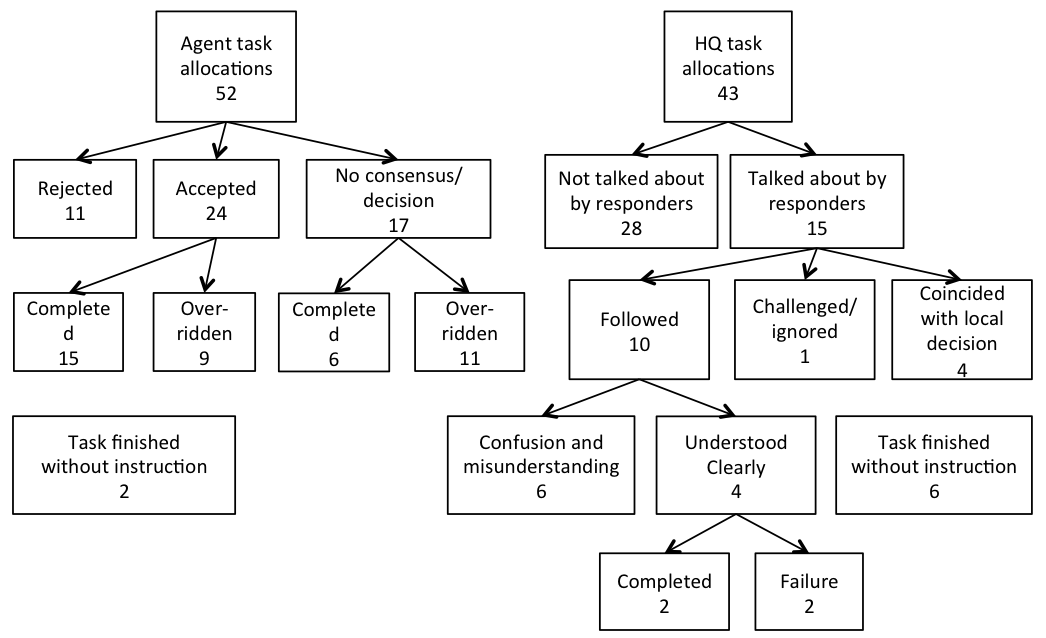
\includegraphics[width=\columnwidth]{message_handling.png}
%\label{fig:msgs}
%\caption{How task allocations were handled by field responders in the agent version (left) and in the non-agent version (right).}
%\end{figure}
%
%\paragraph{Rejecting task allocations}
%
%Field responders rejected the agent's task allocation 11 times in the agent version. All of the rejections happened when the task allocation would have split existing teams, or instructed responders to team up with physically more distant responders. In most cases (9 out of 11), the rejection triggered re-planning and adjusted the task allocation to become consistent with the responder's current team. In the other 2 cases, rejected the task allocation one more time to receive the desired task allocation. 
%
%Overall, players were more likely to reject plan if their proposed teammates were far away from them. For accepted instructions, the average distance between suggested teammates was 12 metres. For rejected instructions, the average distance between suggested teammates was 86 metres.
%
%\subsubsection{The role of HQ}
%The role of HQ changed in that in the non-agent version HQ was responsible for handling task allocations, whereas task allocation was handled by the agent in the other version. HQ frequently monitored the agent's task allocation in the two agent-supported sessions (57 clicks on `show task' in UI responder status widget). Whereas 43 directives in the non-agent session were task allocations, only 16 out of 68 directives were directly related to task allocations in the agent version. Out of these, HQ reinforced the agent instruction 6 times (e.g., ``SS and LT retrieve 09''), and complemented the agent's task allocation 5 times (``DP and SS, as soon as you can head to 20 before the radiation cloud gets there first''). HQ did `override' the agent instruction in 5 cases.  
%
%In the agent version, the majority of HQ's directives (52 out of 68) and assertives (49 out of 51) focussed on providing situational awareness and safely routing the responders to avoid exposing them to radiation. For example, ``Nk and JL approach drop off 6 by navigating via 10 and 09.'', or ``Radiation cloud is at the east of the National College''. 
%
%\subsubsection{Summary}
%The results suggest three key observations with regard to mixed-initiative coordination in the trial:
%
%\begin{itemize}
%\item Field responders performed better (rescued more targets), and maintained higher health levels when supported by the agent.
%\item Rejecting tasks was a frequently employed method to to trigger re-planning to obtain new task allocations aligned with responder preferences.
%\item When task allocation was handled by the agent, the human HQ could focus on providing vital situational awareness to safely route field responders around danger zones; thus demonstrating division of labour and complementary collaboration between human and agent.
%\end{itemize}
%
% 
%%Joel and Wenchao
%%\begin{enumerate}
%%\item Explain setup of experiment - area of interest + setup of tasks
%%\item Explain evaluation = quantitative and qualitative.
%%\end{enumerate}
%%\paragraph{Metrics}
%%\begin{itemize}
%%\item{Comparisons between with/without agent versions for the below:}
%%\item{Performance of FR: number of tasks completed, time on task?, number of messages sent, number of teams formed and disbanded, time on team, acknowledgements of tasks}
%%\item{Messages: classification}
%%\item{Health}
%%\item{Distance travelled}
%%\item{HQ: number of agent monitoring actions (clicks), number of 'supporting'/related messages (e.g., enforcement, contradictions/overriding)}
%%\item{Agent performance: number of instructions, number of replanning steps, replanning robustness (diversion of task allocation compared to previous step)}
%%\item{Following instructions ('obedience'): number of instructions followed vs. not followed (incl. number of HQ interventions/overriding agent allocation), instruction handling diagram}
%%\item
%%\end{itemize}

\vspace{-2mm}
%%\section{Conclusions}\label{sec:conclusions}
%\noindent In this paper developed and evaluated a task planning agent using a mixed-reality game  called AtomicOrchid in order to focus on the issues that arise in human-agent collaboration in team coordination under uncertainty. Results from our study indicate  the planning agent instructed players to carry out successful plans (outperforming a no-agent setting in terms of tasks completed and responders unharmed). Finally our results  suggest that systems involving human-agent collaboration should be adaptive, involve simple  interactions between humans and agents, and allow for flexible autonomy. 
%Future work will look at running AtomicOrchid with expert responders and  exploring different interactional arrangements of humans and agents, in particular where control may be distributed across the team.\vspace{-1mm}
\section*{Acknowledgements}
This work was carried out as part of the ORCHID project funded by EPSRC (EP/I011587/1). 
\bibliographystyle{abbrv}
{
\small
\bibliography{citations}
}


\end{document}
